\documentclass[a4paper, 10pt]{article}

\usepackage[english]{babel}
\usepackage[utf8]{inputenc}
\usepackage{amsmath}
\usepackage{graphicx}
%\usepackage[colorinlistoftodos]{todonotes}
%\usepackage{fullpage}
%\usepackage{siunitx}
\usepackage{microtype}
\usepackage[numbered,framed]{mcode}
\usepackage{url}
\usepackage{float}
\usepackage[noisbn]{babelbib}
\usepackage{epstopdf}
\usepackage{tikz}
\usepackage{breqn}
\usepackage{pdflscape}
\usepackage{units}
\usepackage[toc,page]{appendix}

\usepackage{authblk}

\usepackage{subcaption}
\usepackage{mathtools}
\usepackage{color}
\usepackage{wrapfig}
\usepackage{booktabs}
\usepackage{fancyhdr}
\usepackage{tikz}
\usetikzlibrary{calc}
\usetikzlibrary{patterns}
\usetikzlibrary{decorations.pathmorphing}
\usetikzlibrary{decorations.markings}

\usepackage{tabu}

%\usepackage{rotating}

\bibliographystyle{ieeetr}


\usepackage{geometry}
 \geometry{
 a4paper,
 total={170mm,257mm},
 left=20mm,
 top=20mm,
 }




%\usepackage{marginnote}

\usetikzlibrary{arrows}

\usepackage{listings}
\lstset{language=Matlab}
\lstset{tabsize=2}

\usepackage{verbatim}
\usepackage{amsfonts}

%\sisetup{locale = FR}

\usepackage[pdftex, pdfauthor={}, pdftitle={Wind turbine design}]{hyperref}
% * <d.passed@libero.it> 2015-11-30T20:09:54.849Z:
%
% ^.
\DeclareMathOperator{\sinc}{sinc}
\lstset{inputencoding=latin1}
\lstset{literate=
  {á}{{\'a}}1 {é}{{\'e}}1 {í}{{\'i}}1 {ó}{{\'o}}1 {ú}{{\'u}}1
  {Á}{{\'A}}1 {É}{{\'E}}1 {Í}{{\'I}}1 {Ó}{{\'O}}1 {Ú}{{\'U}}1
  {à}{{\`a}}1 {è}{{\'e}}1 {ì}{{\`i}}1 {ò}{{\`o}}1 {ù}{{\`u}}1
  {À}{{\`A}}1 {È}{{\'E}}1 {Ì}{{\`I}}1 {Ò}{{\`O}}1 {Ù}{{\`U}}1
  {ä}{{\"a}}1 {ë}{{\"e}}1 {ï}{{\"i}}1 {ö}{{\"o}}1 {ü}{{\"u}}1
  {Ä}{{\"A}}1 {Ë}{{\"E}}1 {Ï}{{\"I}}1 {Ö}{{\"O}}1 {Ü}{{\"U}}1
  {â}{{\^a}}1 {ê}{{\^e}}1 {î}{{\^i}}1 {ô}{{\^o}}1 {û}{{\^u}}1
  {Â}{{\^A}}1 {Ê}{{\^E}}1 {Î}{{\^I}}1 {Ô}{{\^O}}1 {Û}{{\^U}}1
  {œ}{{\oe}}1 {Œ}{{\OE}}1 {æ}{{\ae}}1 {Æ}{{\AE}}1 {ß}{{\ss}}1
  {ç}{{\c c}}1 {Ç}{{\c C}}1 {ø}{{\o}}1 {å}{{\r a}}1 {Å}{{\r A}}1
  {€}{{\EUR}}1 {£}{{\pounds}}1
}

\font\myfont=cmr24
\title{\myfont Wind turbine design}



\date{01.04.2016}

% 


\begin{document}
    \begin{figure}[H]
    \centering
    
\includegraphics[width=9cm]{Images/TU-Delft_logo.png}
    \end{figure}


	\begin{center}
    {
    \textbf
    {TU Delft\\
     Wind Turbine design}
    }
    
    
	\end{center}
    
    \vspace{10 mm}

	\begingroup
    	\let\newpage\relax
    	\maketitle
	\endgroup
	
    \vspace{10 mm}
    
    \newpage

 \begin{abstract}


%TODO

    \end{abstract}

\thispagestyle{empty}

\newpage

\tableofcontents

\newpage

\newpage

\section{Introduction}

The Republic of South Africa (RSA), often considered as the \textit{Powerhouse of Africa}, is facing many power outages or shortages of energy mainly due to the lack of investment in power infrastructure \cite{southafrica}. The RSA government is embarking on various energy and efficiency initiatives with a focus on off-grid solutions and renewable energy. The country aspires to raise an industrial revolution to shift towards a \textit{Green Economy} with the intent of boosting its manufacturing industry. This has attracted many large investors in the renewable energy sector, with the likes of Google funding Africa’s largest solar farm project in South Africa \cite{southafricarenew}.

Furthermore, the country’s ample wind resource, especially in the Western Cape and Eastern Cape regions, as seen in Figure \ref{fig:windrs} below, make it a suitable market location for the wind energy industry. Several large scale wind farms have been installed, are under construction or have been planned since 2014. The creation of the South African wind energy industry creates a market for wind turbines that are suitable for this area \cite{southafricawind}. The wind turbine designed and presented in this report will therefore be aimed at the onshore wind energy market in the Southern African region.

Most wind farms in the RSA use turbines rated between 1 and 3 MW with the most recent projects leaning towards using larger turbines of at least 2 MW. Some recent projects include \cite{southafrica}:
\begin{itemize}
    \item the Dorper WF Wind Farm, with 40 Nordex N100 Turbines rated at 2.5 MW
    \item the Dassiesklip Wind Farm, with 9 Sinovel SL3000 turbines rated at 3 MW (under construction)
    \item the Grassridge Wind Farm, with 20 Vestas V112 turbines rated at 3 MW, online since June 2015
\end{itemize}

 Considering the currently employed turbines in South Africa, the new design of turbine for this market will be adjusted so as to obtain the best economic performance; although, it is expected to fall in the power rating range of the above mentioned turbines.

%\begin{center}
\begin{figure}[H] 
%\hspace*{0}
\centering
\begin{subfigure}{0.45\textwidth}
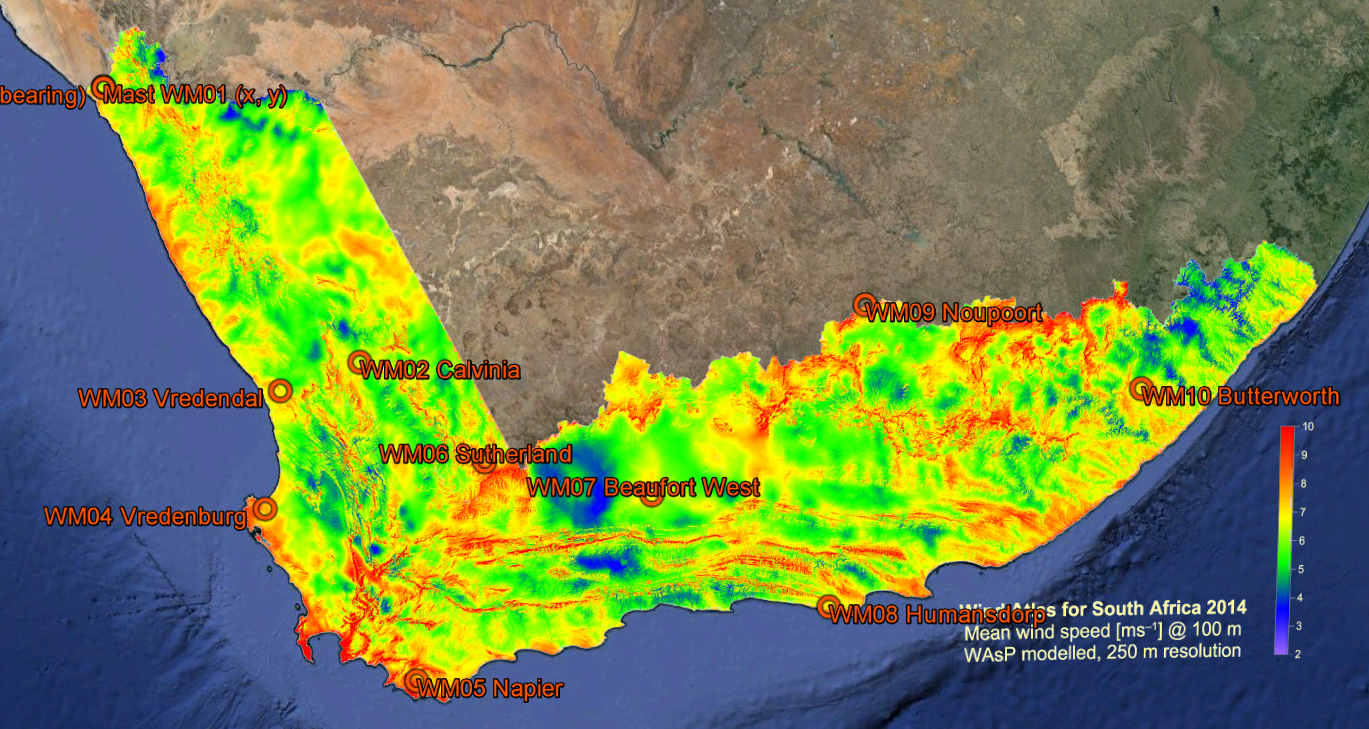
\includegraphics[width=\linewidth]{Images/Wind_atlas_map.PNG} 
\caption{South Africa}
\label{fig:windsa}
\end{subfigure}~
\begin{subfigure}{0.423\textwidth}
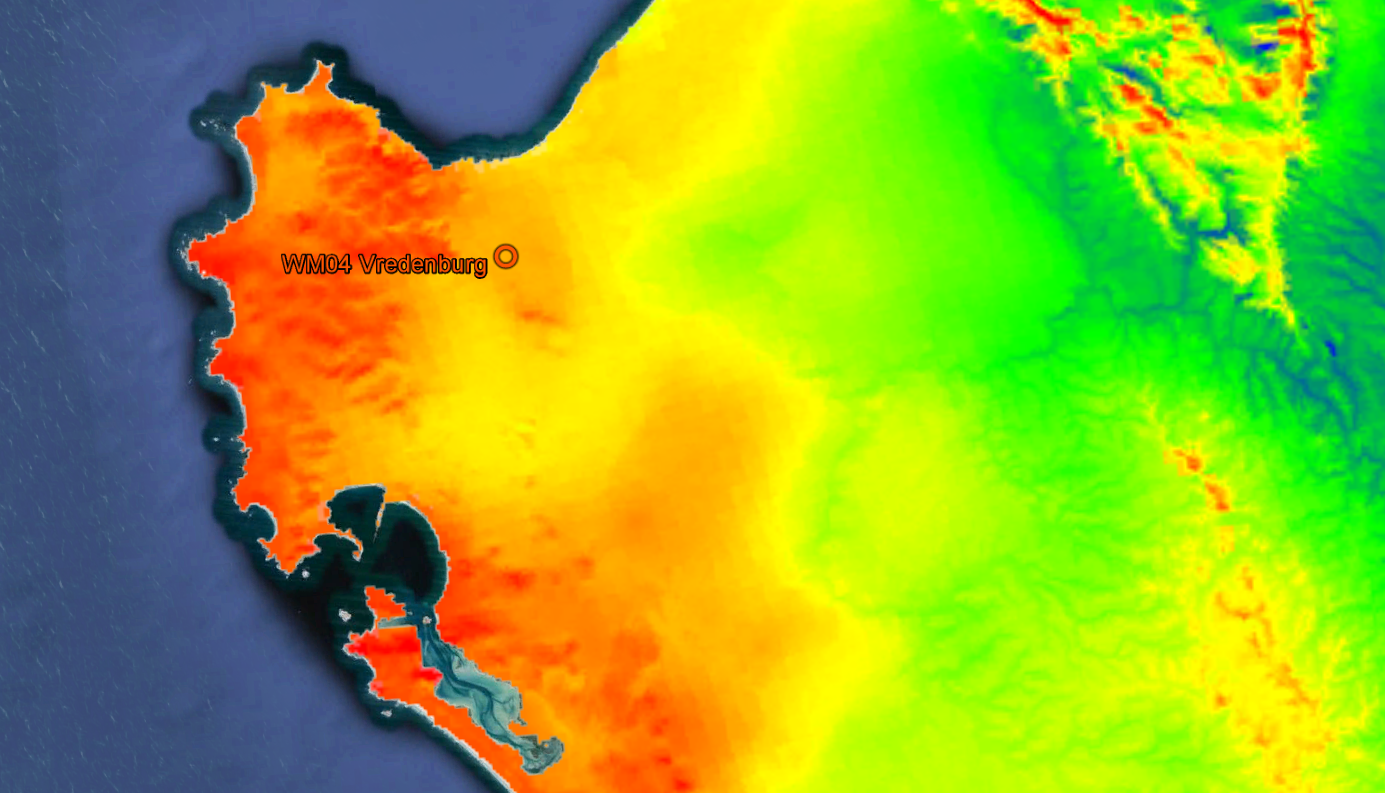
\includegraphics[width=\linewidth]{Images/Wind_atlas_zoomed.PNG}
\caption{Western Cape}
\label{fig:windlocation}
\end{subfigure}
\caption{Wind resources}
\label{fig:windrs}
\end{figure}
%\end{center}

There are currently planned projects for both onshore and offshore wind farms, thought the investment cost of a new offshore farm is still very high, on average in the range of 2.0 to 2.2 million €/MW. The construction of such a wind farm is today only possibly with the support of the government \cite{offcost}. The majority of wind turbines in South Africa today are located in the western and eastern cape regions as these areas have good wind resources. The current energy price has been found to have an average of 0.619 zar/kWh equal to 0.034 €/kWh \cite{eprice} which is an indicator for later discussion regarding the economic potential of the new wind turbine.

For assistance in the calculations of the new turbine, a 5 MW reference turbine is being used \cite{5MW}. This reference has been used to make a first assumption of size and constraints through scaling. It has also been used for guidance in the choice of design parameters and structural design.


\section{System design}

\subsection{Summary of the design}


\begin{center}
Table 21. Objectives and boundary conditions\\
\begin{tabular}{ |l|c| } 
\hline
\textbf{Parameter} & \textbf{Value/Description}  \\ 
\hline
Onshore or Offshore & Onshore  \\ 
\hline
Type of location & Shrubs \\ 
\hline
Wind conditions: Weibull scale factor & 7.5734 \\
\hline
Wind conditions: Weibull shape factor & 2.1416 \\
\hline
Noise constraint (max tip speed) & 72.497 m/s \\
\hline
Visual constraint & - \\
\hline
\end{tabular} \\
\end{center}

\begin{center}
Table 22. Design variables/choices\\
\begin{tabular}{ |l|c| } 
\hline
\textbf{Parameter} & \textbf{Value/Description}  \\ 
\hline
Rated power & 2 MW  \\ 
\hline
Number of blades & 3 \\ 
\hline
Rotor diameter & 96.4 m \\
\hline
Design tip speed ratio & XX \\
\hline
Rotational speed range & XX \\
\hline
Cut-in wind speed & XX \\
\hline
Cut-out wind speed & XX \\
\hline
Rated wind speed & XX \\
\hline
Hub height & XX \\
\hline
\end{tabular}
\end{center}

\subsection{Supporting material, analyses and rationale}

The wind turbine designed and described in this report is made for \textcolor{red}{a location in South Africa (specify)} due to the current interest to increase the energy portfolio through investments in off-grid solutions and renewable sources. The relatively high wind speeds along the coast makes the location a good spot for a wind turbine. The rated power of the wind turbine is set through estimations of a reasonable size of a wind turbine at the established location. For an onshore wind turbine a commonly used size is of a rated power of 2 MW. The number of blades is set to three since turbines with three blades have a slightly higher efficiency than turbines with only two blades and since they are more pleasant for the eye to watch. The reference turbine also have three blades which makes future calculations and comparisons with the reference turbine easier and more accurate.

The turbine is decided to be onshore due to the high cost of an offshore wind turbine project which is currently only feasible with government support. There currently are development projects both onshore and offshore, but according to information retrieved there are no active projects at the chosen location. The maximum tip speed is chosen from noise constraint scaled from the reference turbine for the optimum radius calculated for the new turbine. The calculations for the optimum radius is presented below. (description of location, gives info for visual constraints) 

The wind conditions are determined by the parameters of a Weibull distribution for the 10-minute averaged wind speed. This is done by the use of wind data retrieved from the site at a hub height of 62 m, the highest high with available data. These parameters are thereafter used to compute the wind distribution for each hour. The wind distribution is used to give the energy yield as a function of the theoretical power curve according to Equation \ref{eq:E}. The power curve is computed according to Equation \ref{eq:P} as a function of the radius. The radius is varied from $30 m$ to $120 m$. The equations for energy yield and the power curve is thereafter solved simultaneously to find the variation of the energy yield for different values of the radius. To determine the optimal radius, the normalised cost over energy yield has been computed, assuming that the normalised total cost for onshore wind turbines can be calculated using Equation \ref{eq:C}.

\\
\begin{equation}
E_{y}\ = \sum_{i} P_{i}\, h_{i}\, \Delta \, v
\label{eq:E}
\end{equation}

\begin{equation}
P = \frac{\pi\, \mathrm{Cp}\, R^2\, \rho\, v^3}{2}
\label{eq:P}
\end{equation}

\begin{equation}
C_{norm}\ = 0.7 + 0.3 {\left(\frac{D}{D_{ref}}\right)}^{2.6}
\label{eq:C}
\end{equation}

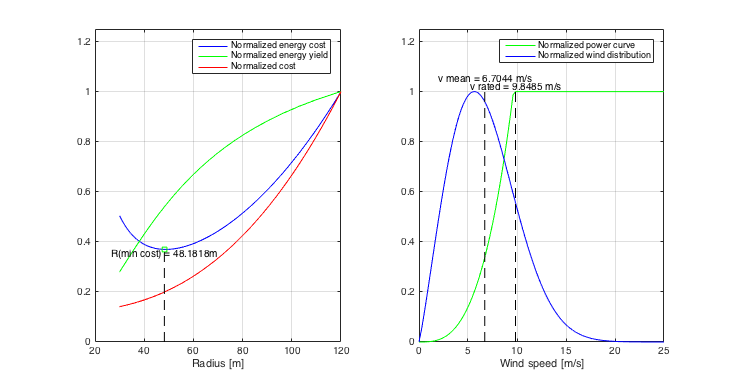
\includegraphics[width=15cm]{Images/op_radius.png}\\

\section{Rotor aerodynamic and structural design} \label{rotor design}
This section deals with the aerodynamic and the inner structural design of the blades for the on-shore wind turbine to be designed at the tip-speed ratio of $7.36$ and for a rotor diameter of $96.36\ m$, as decided in Section \ref{system design}. 
\subsection{Summary of the design}
\begin{table}[H]
\begin{center} 
\caption{Objectives and boundary conditions}\label{tab:rotordesign2}
\begin{tabular}{ |l|c| } 
\hline
\textbf{Parameter} & \textbf{Value/Description}  \\ 
\hline
Number of blades & 3  \\ 
\hline
Rotor diameter & 96.36 m \\ 
\hline
Design tip speed ratio & 7.36 \\
\hline
\end{tabular} \\
\end{center}
\end{table}

\begin{table}[H]
\begin{center} 
\caption{Objectives and boundary conditions}\label{tab:rotordesign2}
\begin{tabular}{ |l|c| } 
\hline
\textbf{Parameter} & \textbf{Value/Description}  \\ 
\hline
Aerofoil 1 & XX  \\ 
\hline
Min. and max. dimensionless radius r/R for aerofoil 1 & XX \\ 
\hline
Aerofoil 2 & XX \\
\hline
Min. and max. dimensionless radius r/R for aerofoil 2 & XX \\
\hline
Aerofoil 3 & XX \\
\hline
Min. and max. dimensionless radius r/R for aerofoil 3 & XX \\
\hline
Twist offset at tip (= blade pitch angle for optimal operation) & XX \\
\hline
‘Thickness factor’ of the blade laminates & XX \\
\hline
\end{tabular} \\
\end{center}
\end{table}


Figure 31. Chord distribution\\

Figure 32. Twist distribution\\

\subsection{Supporting material, analyses and rationale}
The blade from the NREL $5\ MW$ reference turbine \textcolor{red}{(cite this)} is designed using an optimised chord and twist distribution based on its design parameters. The design is then compared with the original reference turbine.

The blade is scaled using the scaling laws from the NREL $5\ MW$ to the desired $2\ MW$ wind turbine. The scaling laws used for each of the parameters have been shown in Table (\textcolor{red}{show table for scaling laws}). These scaling laws are obtained from the square-cube law which states that (\textcolor{red}{state the square-cube law}) and by referring to the scaling laws provided with the course material (\textcolor{red}{cite scaling laws}). The blade's geometry is then optimised to obtain the best desirable performance measured by maximising the power coefficient $C_p$, as can be seen in listing \ref{lst:task3_2} of appendix A.

The optimisation's target is to obtain the twist and chord distribution functions that produce the highest $C_p$ under some constraints. Such functions are expressed by using a set of degrees of freedom, which represent the values of twist and chord at certain uniformly distributed radial locations. The values at all the other locations are obtained by means of cubic spline interpolation. The radial locations used to evaluate the value of $C_p$ are linearly scaled from the reference NREL $5\ MW$ turbine.

The value of $C_p$ is computed by using the BEM code available in the FAST program. Such code has been extracted and isolated as a function that returns the value of $C_p$ given the properties of the wind turbine, as can be seen in listing \ref{lst:Cp}.


The outer geometry of a rotor blade is thus defined. In order to obtain the interior structure the mass and stiffness of the blades, which make up the structural properties, are scaled from the NREL $5\ MW$ reference turbine using the scaling laws shown in Table (\textcolor{red}{show table for scaling laws}). The scaled blade structural properties are utilised to calculate the tip deflection of the blade designed for the new $2 MW$ wind turbine. In order to calculate the tip deflections both the reference blades and the optimised blades were loaded at a wind speed $v=9.84\ m/s$, which is the rated wind speed for the $2\ MW$ wind turbine.

The tip deflection is calculated using a simple finite element model. The model is based on the Bernoulli beam theory which is applied to the blade modelled as a cantilever beam. The blade discretized using the beam theory is shown in Figure (\textcolor{red}{show beam_theory discretized figure}).The equations for moment and deflection obtained from the Beam theory are applied for each section. Upon using the model the deflections in the flap-wise and the edgewise direction are shown in Figure (\textcolor{red}{show deflection plots}).It can be observed from the plots that, the deflections for the new blade are smaller than that for the reference blade in the flap-wise direction. They are however seen to have increased in the edgewise direction. This is due to the differences in the chord and twist distribution observed between the optimised and the scaled reference blades, as shown in Figure (\textcolor{red}{show deflection comparison plots}). The new chord and twist distributions in the optimised blade cause a redistribution in the inertia in the flap-wise and edgewise directions. Thus, the deflections in the flap-wise and edgewise directions change as a consequence. 

The stresses developed in the flap-wise and edgewise directions in the $5\ MW$ reference and $2\ MW$ optimised turbines are compared relatively by making use of their ratios. The properties that the stresses depend on are namely, the mass $M$ and the stiffness $EI$ along the direction being considered. An additional scaling factor used is the chord $c$ of the respective blades. The chord is utilised to factor in the relative changes in the sizes of the blade cross-sections. The dependence of the stresses for the reference and optimised blades on these factors are expressed as,

\begin{align}
    \sigma_{ref} &\propto \dfrac{M_{ref}}{EI_{ref}}\cdot c_{ref} \label{eq:stress_ref} \\
    \sigma_{opt} &\propto \dfrac{M_{opt}}{EI_{opt}}\cdot c_{opt} \label{eq:stress_opt}
\end{align}

where, $\sigma_{ref},\ M_{ref},\ EI_{ref}$ and $c_{ref}$ represent the stress, mass, stiffness and the chord respectively of the reference blade for the  $5\ MW$ turbine. Similarly, $\sigma_{opt},\ M_{opt},\ EI_{opt}$ and $c_{opt}$ represent the stress, mass, stiffness and the chord respectively of the optimised blade for the  $2\ MW$ turbine being designed. The relationship between the two stresses is established by taking the ratio between Equation \ref{eq:stress_opt} and Equation \ref{eq:stress_ref} and is expressed as,

\begin{equation}
     \zeta = \dfrac{\sigma_{opt}}{\sigma_{ref}} = \dfrac{M_{opt}}{M_{ref}}\cdot\dfrac{EI_{ref}}{EI_{opt}}\cdot \dfrac{c_{opt}}{c_{ref}}
\label{eq:stress_ratio}
\end{equation}

The stress ratio shown in Equation \ref{eq:stress_ratio} is calculated for both the edgewise and the flap-wise directions.

\section{Drive train design}

The following section deals with the design of the drive train and involves the selection of a type of drive train and the calculation of the component specifications therein.

\subsection{Choice of drive train}

The choice of drive train configuration for the wind turbine is made by weighing advantages and disadvantages of various types of typical drive trains and relating them to the market location and desired conditions. A list of advantages and disadvantages of the four most common drive train configurations are listed in Table \ref{tab:comparison_dt}. 

\begin{table}[H]
\label{tab:comparison_dt}
\hspace*{-2.cm}
\centering
\caption{Comparison of drive train concepts}
\begin{tabular}{ |l|l|l|l| }
 \hline
 \textbf{Drivetrain} & \textbf{Advantages} & \textbf{Disadvantages} & \textbf{Specifications} \\ 
 \hline
 Doubly Fed & - Suitable for 2 MW & - Gear failures and & - Pitch control\\ 
  Induction & rated power &  maintenance costs & - For rated\\ 
 (Geared) & - Variable speed & - Generator with & power between\\
  & generator & brushes & 1.5 – 3 MW\\
  & - Active- and & & \\
  & reactive-power control & &\\
  & - Only about a &  & \\
  & third of the power &  & \\
  & flows through inverter & & \\
  & \to\,$smaller inverter & & \\
  & \to\,$lower inverter & & \\
  & cost and losses & & \\
  & - Controlled voltage & & \\
  & and frequency & & \\
  \hline
  Full Conversion & - Good power quality & - Large and heavy & - Pitch control\\
  Permanent Magnet & - Possibility of & - Difficult to transport & For rated power \\
  (Geared on non-) & omitting gearbox & & between 2 – 4 MW \\
  \hline
 Full Conversion High & - Very good & - Complex cooling & - Pitch control\\
 Temperature & power quality & of generator & - For rated power\\
 Superconducting & - Efficient at all loads & - Large torque load & above 5 MW\\
 (Direct Drive) & - Small & & \\
  & - Light & & \\
  & - No gearbox & & \\
  & - Control system can & & \\
  & be adapted to & & \\
  & facilitate operation & & \\
  & on weak grids & & \\
  \hline
  Constant Speed & - Simple design & - Low power quality & - Stall control \\
   & - Lower & - Low control of & - Typically for  \\
   & manufacturing costs & frequency and voltage & rated power below \\
   & & - Narrow range of & 1.5 MW \\
   & & efficient rotational & \\
   & & speed & \\
   & & - Higher cut-in & \\
   & & wind speed & \\
  \hline
 \end{tabular}
\end{table}

\newpage
Although constant speed (CS) drive train turbines have a simple design, due to the lack of speed control systems they have numerous drawbacks that limit their applicability in the Southern African market, even though it makes them cheaper. They produce low power quality as their frequency and voltage is not well controlled, thus requiring a stiff grid. However, particularly in South Africa, the grid is recognisably weak \cite{onishi}. Additionally, CS drive trains are typically used for turbines with a rated power below 1.5 MW, and thus can be ruled out of the options  \cite{mcgahan}.

The full conversion high temperature superconducting (HTS) drive train generates a very good quality power and can be designed small, light and without a gearbox. For these reasons it would be an attractive configuration for Southern Africa where the turbines would have to be transported to the wind farm locations via roads of questionable standards. Nevertheless, full conversion HTS direct drive trains are typically applied for turbines with a rated power above 5 MW and thus can be ruled out as not being suitable for the 2 MW AlphaWind turbine \cite{mcgahan}.

Full conversion permanent magnet (PM) type generators can have direct or geared drive trains and produce good quality power. In cases no gearbox is used, a bulky multipole direct driven generators are used. These are large and thus difficult to transport thus counteracting the benefit of the gear-less configuration \cite{hansen}.

The doubly fed induction generator (DFIG) configuration uses a transmission with a gearbox; however, the output power quality is relatively good as it has a voltage and frequency control. Additionally, the partial frequency converter allows using a smaller and cheaper inverter with lower losses as only about 30\% of the power produced goes through the inverter \cite{hau}. The generator is not particularly bulky as in direct drive trains and can easily be transported to the installation locations. The rated power of the AlphaWind turbine falls well between the range of power for which DFIG is typically applied. Furthermore, considering that power quality and transportability are two very important factors in the choice of drive train for the Southern African region, the DFIG configuration is the most suitable and will thus be applied in the AlphaWind turbine.


\subsection{Main frame and electrical system configuration}

\subsubsection{Summary of the design}


\begin{center}
Table 41. Objectives and boundary conditions\\
\begin{tabular}{ |l|c| } 
\hline
\textbf{Parameter} & \textbf{Value/Description}  \\ 
\hline
Special considerations for the chosen system design & XX  \\ 
\hline
\end{tabular} \\
\end{center}


Figure 41. Overview of nacelle

\subsubsection{Supporting material, analyses and rationale}

\newpage

\subsection{Gearbox}

\subsubsection{Summary of the design}

The summary of the gearbox design is given in Table \ref{tab:overview_drivetrain} and \ref{tab:gearbox_config}. 

\begin{table}[h]
\centering
\caption{Overview of the drivetrain}
\label{tab:overview_drivetrain}
\begin{tabular}{ |l|c|c| } 
\hline
\textbf{Parameter} & \textbf{Symbol} & \textbf{Value/Description}\\ 
\hline
Speed range at rated power (LSS / HSS) & $n_{LSS}$/$n_{HSS}$&  14.36 rpm / 1077 rpm \\ 
\hline
Torque at rated power (LSS / HSS) & $Q_{LSS}$ / $Q_{HSS}$ & 1410696 Nm / 18253 Nm\\
\hline
Mass of the gearbox & $m_{gearbox}$ & 17.4 t\\
\hline
\end{tabular} \\
\end{table}

\begin{table}[h]
\centering
\caption{Gearbox configuration}
\label{tab:gearbox_config}
\begin{tabular}{ |l|c|c| } 
\hline
\textbf{Parameter} & \textbf{Symbol} & \textbf{Value/Description}\\ 
\hline
Gearbox type & & 3 stage gearbox\\
\hline
Gearbox stage 1 & & planetary\\
\hline
Gearbox stage 2 & & parallel\\
\hline
Gearbox stage 3 & & parallel\\
\hline
Gearbox ratio & N & 75 \\
\hline
Gear ratio stage 1 & $N_1$ & 5\\
\hline
Gear ratio stage 2 & $N_2$ & 5\\
\hline
Gear ratio stage 3 & $N_3$ & 3\\
\hline
Number of teeth sun& $z_{sun1}$ & 20\\
\hline
Number of teeth planet& $z_{planet3}$ & 30\\
\hline
Number of teeth ring& $z_{ring3}$ & 80\\
\hline
Number of teeth pinion& $z_{p2}$ & 20\\
\hline
Number of teeth gear& $z_{g2}$ & 100\\
\hline
Number of teeth pinion& $z_{p3}$ & 20\\
\hline
Number of teeth gear& $z_{g3}$ & 60\\
\hline
\end{tabular} \\
\end{table}

\subsubsection{Supporting material, analyses and rationale}

The torque on the low speed shaft (LSS) needed to generate 2 MW of rated power can be found using the mechanical power on the LSS and the rated angular frequency as
\begin{equation}
    Q_{LSS} = \dfrac{P_{LSS\, rated}}{\omega_{rated}}
    \label{eq:Q_LSS}
\end{equation}
where $P_{LSS}$ is the rated power augmented by the overall drivetrain efficiency. 

The gearbox is designed as a three stages multistage gearbox with the first stage being planetary and the second and third stage being parallel stages. With this an overall gearbox ratio of 75 is achieved. 
The weight of the gearbox is estimated using the following empirical formula

\begin{equation}
    m_{gearbox} = 70.94 \cdot Q_{LSS}^{0.759}
\end{equation}
where $Q_{LSS}$ is the rated LSS torque given by Equation \ref{eq:Q_LSS} inserted in kNm \cite{Fingersh2006}. With this the mass of the gearbox was estimated as

\begin{align}
m_{gearbox} = 17.4 \, t
\end{align}


\subsection{Generator}

\subsubsection{Summary of the design}

The summary of the generator design is given in Table \ref{tab:generator_config}. 
\begin{table}[h]
\centering
\caption{Generator configuration}
\label{tab:generator_config}
\begin{tabular}{ |l|c|c|} 
\hline
\textbf{Parameter} & Symbol & \textbf{Value/Description}  \\ 
\hline
Type of generator & & DFIG\\
\hline
Power rating & & 2.105 MVAr\\
\hline
Generator power factor & pf & 0.95\\
\hline
Grid frequency & $f_{grid}$ & 50 Hz  \\
\hline
Generator poles & $p$ & 6\\
\hline
Generator voltage level & $U_{gen}$ & 1400 V\\
\hline
Generator torque at rated speed & $Q_{HSS}$ & 18253 Nm \\
\hline
Minimum generator speed & $n_{min}$ & 567 rpm\\
\hline
Synchronous speed & $n_s$ & 1000 rpm\\
\hline
Generator rated speed & $n_{rated}$ & 1077 rpm\\
\hline
Maximum generator speed & $n_{max}$ & 1250 rpm \\
\hline
Force density & $F_d$ & 30000 $\frac{N}{m}$\\
\hline
Generator volume & $V_{gen}$ & 0.3042 $m^3$\\
\hline
Generator length & $L_{gen}$ & 1 m\\
\hline
Rotor radius & $R_{rot}$ & 0.3111 m\\
\hline
Rotor mass & $m_{rot}$ & 2388 kg \\
\hline
Inertia generator rotor & $\Theta_{rot}$ & 122.5 $kg m^2$\\
\hline
Generator inverter rating & $x$ & 0.25\\
\hline
Safety margin against rotor overshoot & & 16 \%\\
\hline
\end{tabular} \\
\end{table}

\subsubsection{Generator design}

The choice of DIFG for the AlphaWind design offers the advantage to operate at a wide range of generator speeds with high efficiency. DFIG generators can be operated in voltage control mode (PV) and power factor control mode (PQ) \cite{Londero2012}. Since the turbine is variable speed and thus delivers dependent on the wind speed different amount of power to the grid, the DFIG generator is operated in PV mode with a power factor specified at 0.95. The mechanical power needed to get a desired amount of electrical power out of the turbine is calculated as

\begin{equation}
    P_{in} = \dfrac{P_{out}}{\eta_{el}\eta_{s1}\eta_{s2}\eta_{s3}} + P_{loss\,fix}
    \label{eq:P_in}
\end{equation}
\\
where $\eta_{el}$ is the efficiency of the generator and all the other components together (bearings), $\eta_{si}$ are the efficiencies of the gearbox stages (variable loss) and $P_{loss, \, fix}$ are the fixed losses in the gearbox stages independent of the transmitted power.


The the efficiency of the generator together with the bearings is assumed to be constant
\begin{align}
    \eta_{el} = 0.9715
\end{align}

With this the input needed into the generator to produce 2 MW of rated power becomes

\begin{align}
    P_{in\,gen} = \dfrac{P_{rated}}{\eta_{el}} = \dfrac{2 MW}{0.9715} = 2.05 MW
\end{align}

At rated speed each gearbox stage is assumed to have 1\% loss of transmitted power \cite{hau}. This means an efficiency of $\eta_{ri} = 0.9900$ at rated power for each stage, where half of it is assumed to be independent of the transmitted power and half of it is assumed to be a linear function of the transmitted power. With this the fixed loss of the gearbox is calculated at rated power as half of the sum of the losses in each stage: 

\begin{align}
    P_{loss\,fix} &= \dfrac{1}{2} \sum \limits_{s = 1}^{3} \left( P_{in} - P_{out}\right)_{s}\\
    &= \dfrac{1}{2} \left( \left( \dfrac{P_{in\,gen}}{\eta_{r1}\eta_{s2} \eta_{r3}} - \dfrac{P_{in\,gen}}{\eta_{r2} \eta_{r3}} \right)_{1} + \left( \dfrac{P_{in\,gen}}{\eta_{r2} \eta_{r3}} - \dfrac{P_{in\,gen}}{\eta_{r3}}\right)_{2}+ \left( \dfrac{P_{in\,gen}}{\eta_{r3}} - P_{in\,gen} \right) \right)\\
    &= \dfrac{1}{2} \left( \dfrac{2.05 MW}{0.99^3} - 2.05 MW \right) = 31.5 \,kW
\end{align}

For the losses that vary with the power in Equation \ref{eq:P_in} subsequently a gearbox efficiency of $\eta_{si} = 0.9950$ must be used (since the fixed 0.5 \% loss is accounted via $P_{loss \, fix}$).

With this the overall efficiency of the drivetrain at rated power is

\begin{align}
\eta_{tot, rated} = 0.9430    
\end{align}

The dimensions of the generator rotor are calculated using the formulae given in the lecture. We assume the flux density of the stator windings to be $F_d = 30000 \frac{N}{m}$. With this volume of the rotor is calculated as

\begin{equation}
    V_{rot} = \dfrac{P_{in \, gen}}{2 \omega_{rated} F_d} = \dfrac{2.05 MW}{2 \cdot 112.78 \frac{rad}{s} \cdot 30000 \frac{N}{m}} = 0.3042 \,m^3
\end{equation}

The length of the generator rotor was assumed to be 1 m, with this the generator rotor radius $R_{rot}$ was calculated. Using these dimensions the generator rotor mass is estimated. The overall generator mass (rotor + stator + housing) is calculated using again the empirical formula given in Reference~\cite{Fingersh2006}

\begin{equation}
    m_{generator} = 6.47 P_{rated}^{0.9223}
\end{equation}

where $P_{rated}$ is the rated power of the turbine inserted in kW. 

The generator rotor inertia is calculated using the standard formula for the inertia of a rotor: 

\begin{equation}
\Theta_{rot}= \dfrac{1}{2}m_{rot}R_{rot}^2
\end{equation}

The generator inverter rating, $x$, is used to specify the minimum rotor speed of the generator that is required to start the generator.  







\newpage
\subsection{Inverter}

\subsubsection{Summary of the design}

\begin{table}[h]
\centering
\caption{Inverter design specification}
\label{tab:}
\begin{tabular}{ |l|c|c|} 
\hline
\textbf{Parameter} & Symbol & \textbf{Value/Description}  \\ 
\hline
Voltage level & $U$ & 1.8 kV\\
Power rating & & \\
\hline
\end{tabular} \\
\end{table}


\begin{table}[h]
\centering
\caption{Inverter design}
\label{tab:}
\begin{tabular}{ |l|c|c|} 
\hline
\textbf{Parameter} & Symbol & \textbf{Value/Description}  \\ 
\hline
Location of the converter & & tower base  \\ 
Type of converter & & Air cooled doubly-fed converter \\
Weight of inverter & $m_{inverter}$ & 1900 kg \\
\hline
\end{tabular} \\
\end{table}


\subsubsection{Choice of inverter and design}

As inverter the ACS800-67 conveter by ABB is chosen \cite{ABB}. 

\subsection{Power cables}

\subsubsection{Summary of the design}
The summary of the cable design is given in Table \ref{tab:power_cables}.

\begin{table}[h]
\centering
\caption{Power cables in tower}
\label{tab:power_cables}
\begin{tabular}{ |l|c|c|} 
\hline
\textbf{Parameter} & Symbol & \textbf{Value/Description}  \\ 
\hline
Voltage level & $U$ & 1.8 kV\\
Current per phase & I_{phase} & 101.3 A\\

Cable & & HELUWIND® WK POWERLINE ALU 105°C 1,8/3kV\\

\hline
\end{tabular} \\
\end{table}

\subsubsection{Cable selection}

The cable chosen for inside the turbine tower is the (N)TSCGEHXOEU cable by Draka Industry&Speciality. This three phase cable with Copper cores is specially designed for application in Wind Turbines and certified for 1,8/3 kV at 50Hz \cite{Draka}. This cable is chosen because of it's high flexibility which is needed inside the tower to connect the yawed turbine nacelle to the inverter at the bottom of the tower. 






\section{Tower design}

Once the rotor design has been completed, it is possible to assess the structural properties of the wind turbine's tower. The process is divided in two phases: first, the reference tower is linearly scaled in height, section diameter, and wall thickness. Then, by computing the thrust produced by the rotor, the stresses inside the tower are estimated, and it is checked that the safety factor is satisfactory, and that the fist natural frequency of the system is sufficiently high.

\subsection{Summary of the design}

The final results for the tower analysis are presented in Table \ref{tab:tower}. The minimum safety factor of $3.05$ is considered to be sufficient, as presented in \cite{NREL_tower}.
The first natural frequency is $0.402Hz$. By looking at the frequency ranges of the $1P$ and $3P$ regions, it is noted that possible resonance problems may arise at a rotor speed of $8.0 rpm$. It is thus necessary to apply frequency skipping at such frequency.

\begin{table}[H]
\begin{center} 
\caption{Rotor frequency ranges}\label{tab:freq_ranges}
\begin{tabular}{ |l|c| } 
\hline
\textbf{Parameter} & \textbf{Value/Description}  \\ 
\hline
1P cut-in speed & $0.13 Hz$ \\ 
\hline
1P cut-out speed & $0.24 Hz$ \\ 
\hline
3P cut-in speed & $0.38 Hz$ \\ 
\hline
3P cut-out speed & $0.72 Hz$ \\ 
\hline
\end{tabular} \\
\end{center}
\end{table}


\begin{table}[H]
\begin{center} 
\caption{Tower design parameters}\label{tab:tower}
\begin{tabular}{ |l|c| } 
\hline
\textbf{Parameter} & \textbf{Value/Description}  \\ 
\hline
Tower height & $69.5 m$ \\ 
\hline
Tower bottom radius & $2.38 m$ \\ 
\hline
Tower top radius & $1.53 m$ \\
\hline
Tower top thickness & $0.0214 m$ \\
\hline
Tower bottom thicnkess & $0.0151 m$ \\
\hline
Maximum strees & $81.7883 MPa$ \\
\hline
Minimum safety factor & $3.05$ \\
\hline
First natural frequency & $0.402 Hz$ \\
\hline
\end{tabular} \\
\end{center}
\end{table}

\subsection{Supporting material, analyses and rationale}

In order to compute stresses in the blade, thrust must be computed fist. The highest value of thrust is obtained at the rated wind speed \cite{hau}, thus it is chosen to use such condition to asses the tower design. 
To compute thrust, the BEM code is used again to compute the induction factor $a$. Then, lift and drag distributions are computed, starting from the definition of the angle of attack $\alpha$:

\begin{equation}
    \alpha = \phi - \beta + \theta 
\end{equation}

where

\begin{equation}
    \phi = \arctan\left(\frac{V(1 - a)}{ \Omega r}\right)
\end{equation}

The actual velocity at the blade airfoil is computed as

\begin{equation}
    V = \sqrt{ (V ( 1 - a )) ^ 2 + ( \Omega r ) ^ 2}
\end{equation}

Lift and drag per unit span are computed as

\begin{equation}
    \frac{dL_a}{dr} = \frac{1}{2} \rho V ^ 2 C_l c;
\end{equation}

\begin{equation}
    \frac{dD_a}{dr}  = \frac{1}{2} \rho V ^ 2 C_d c;
\end{equation}

and finally, forces in the edge and flap directions are computed as

\begin{equation}
    \frac{dF_y}{dr}  = dL_a \sin(\phi) - dD_a \cos(\phi);
\end{equation}

\begin{equation}
    \frac{dF_z}{dr}  = dL_a \cos(\phi) + dD_a \sin(\phi);
\end{equation}

The total value of thrust per blade is computed by integrating the force in the $z$ direction

\begin{equation}
    F_z = \int_{0}^{R} \frac{dF_z}{dr} dr
\end{equation}

The final value of thrust is computed at rated conditions

\begin{align}
    T &= 3 F_z \\
    &= 308 kN \\ \nonumber
\end{align}

At this point, stresses are computed in the tower by applying simple beam theory using a dynamic loading factor of $1.35$ and a static loading factor of $1.2$. The sectional properties of the tower and the stresses in the tower's wall are computed as presented in \cite{Bispl} as a function of height $h$, while the material properties are supposed to be equal to those used for the reference turbine. Maximum stresses are supposed to be equal to the summation of gravitational and bending stresses, the latter being the most severe. The value of the stress in the tower is computed as

\begin{equation}
    \sigma = \frac{N}{A} + \frac{M r_{ext}}{I}
\end{equation}

\begin{figure}[H]
\centering
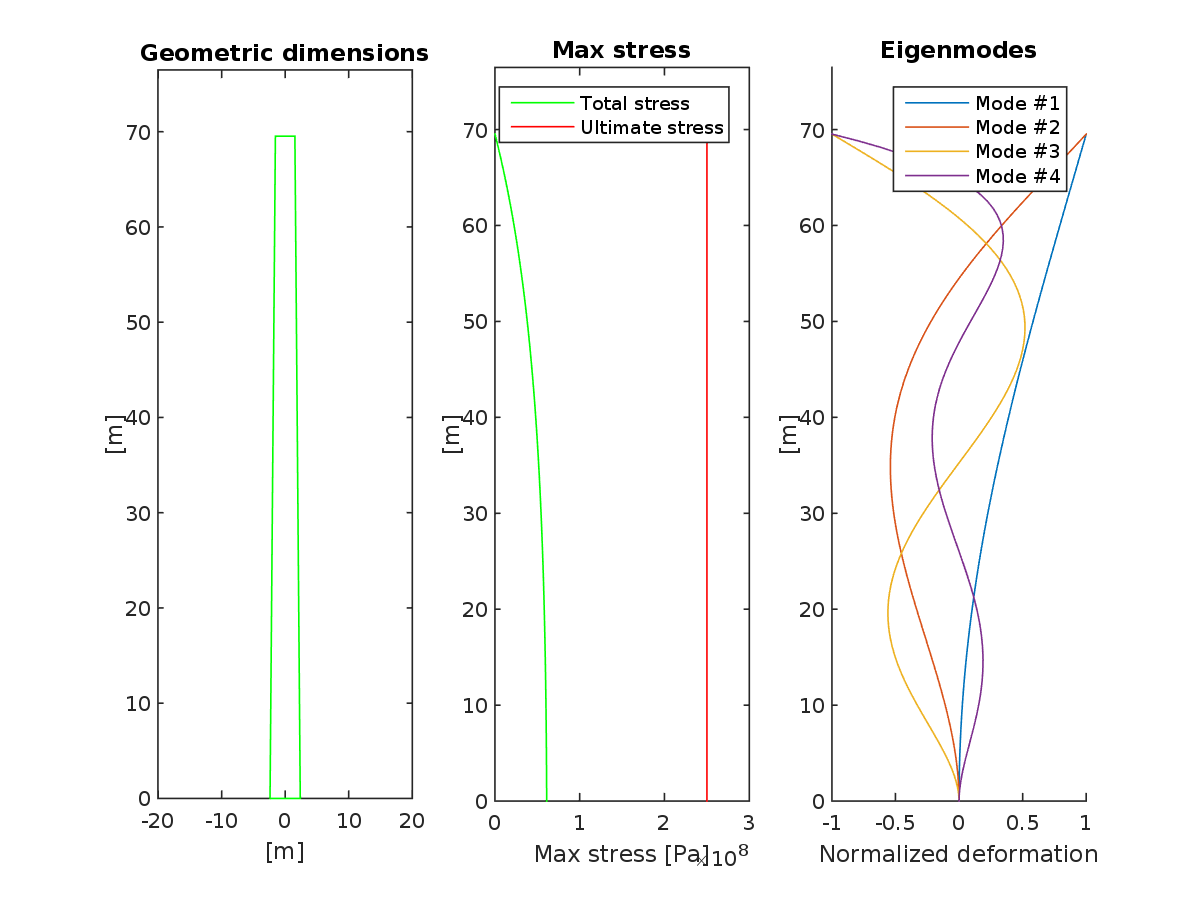
\includegraphics[width=0.9\textwidth]{Images/Tower.png} 
\caption{Tower dimensions, stresses and natural modes}\label{fig:chord}
\end{figure}

From \cite{Bispl} also natural frequencies of the beam are computed, by applying a simple polynomial Galerkin approximation of the Principle of Virtual Work.  

\section{Preliminary analysis and design update}

\subsection{Summary of the design}
\subsection{Supporting material, analyses and rationale}




\section{Control design}

\subsection{Summary of the design}
\subsection{Supporting material, analyses and rationale}

\section{Preparation of load cases and wind conditions}

\subsection{Summary of the preparations}
\subsection{Detailed description of the conditions}

\section{Certification analysis}

\subsection{Summary of the analysis}

\subsection{Detailed description of the analysis and interpretation}

\section{Reflection and prospects}

\addcontentsline{toc}{section}{References}


\bibliography{bibliography}
\nocite{*}



\end{document}
